% !TeX root = ../main.tex
% !TeX spelling = en_GB
% !TeX program = pdflatex

\chapter{Materials and Methods}
\label{chap:methods}

The methods in this chapter can be seen as the answers to research question RQ1-RQ3 from \Cref{chap:intro}. To begin with, a few different light sources and illumination angles were investigated. In section \ref{sec:discussionstarting}, the lighting alternatives that were considered, are described. It was settled that a shadowgraph system with background illumination from an \gls{led} was to be used. The experimental setup was tested using different water droplet generators and a test target consisting of micrometer sized lines and dots. Analyzing the optical system and testing different segmentation algorithms, we found a simple way to define the sample volume for each individual droplet. To test the ability of measuring concentration we needed to build a weather protected prototype that could be used in parallell with a second instrument. The prototype needed to be fully automatic, able to analyze images in real time 24 hours a day for several months and store the results in a compressed format. To calibrate the size measurement and the measurement range, the previously mentioned dots of different sizes were used. The size measurement was also verified using distributions polymer microspheres, applied by blowing compressed air through a glass dispenser.

\section{The Shadowgraph System}

The instrument is a shadowgraph system using a monochrome \gls{cmos} camera with a 4x magnifying telecentric lens and a \gls{led} with a collimating lens illuminating the background. \Cref{fig:shadowprinc} shows a sketch of the system. The system was first tested in the experimental setup seen in \Cref{fig:experimental}. 

\begin{figure}[ht]
\centering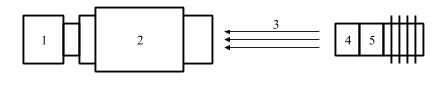
\includegraphics[width=0.75\linewidth]{./figures/shadowprinc.jpg}
\caption{Principle of shadowgraphy. 1. Camera. 2. Telecentric lens. 3. Parallell focused light beam. 4. Collimating lens. 5. \gls{led}.}
\label{fig:shadowprinc}
\end{figure}

The blue \gls{led}, shown to the right in \Cref{fig:experimental}, was initially powered by a SignaTech Strobe Controller from Advanced Illumination. The SignaTech Controller can produce up to 4A at 100V. For the prototype instrument, another current driver, the Picolas LDP-V 10-70 was chosen. This driver can produce short 12A pulses. For controlling the pulse length, a microcontroller is used. 

\begin{figure}[ht]
\centering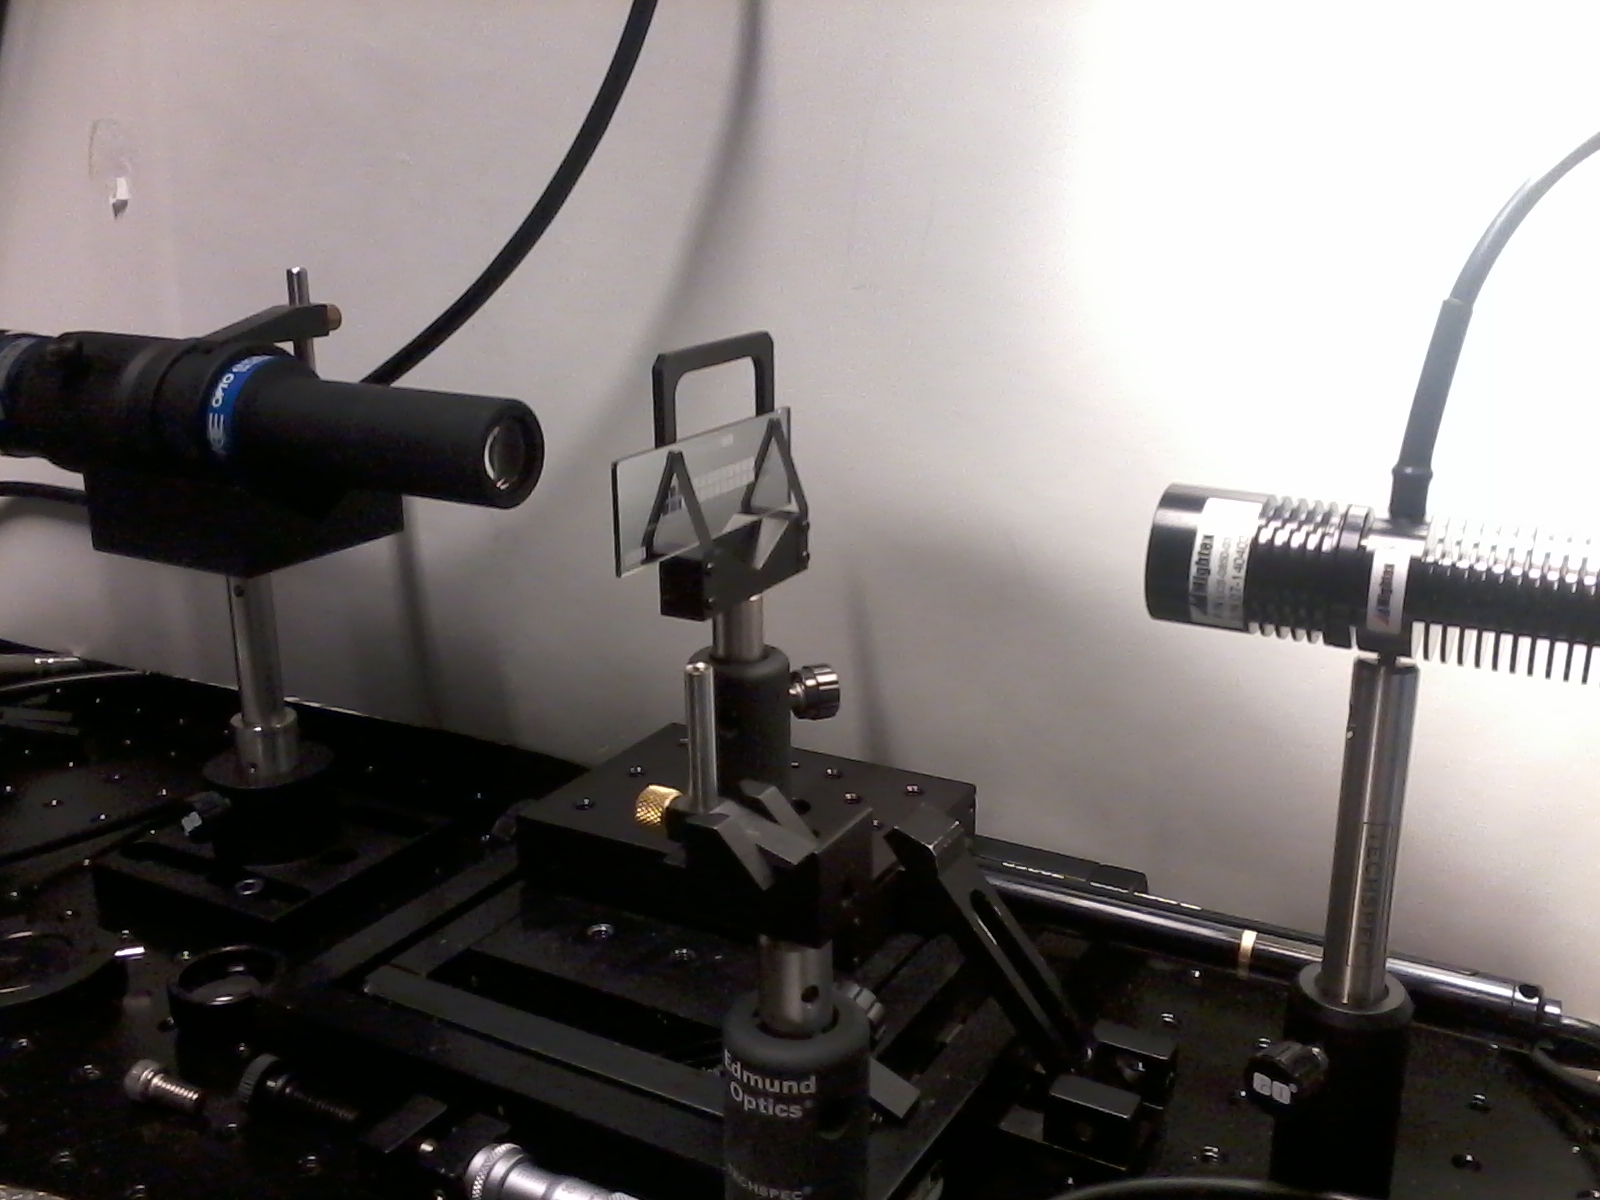
\includegraphics[width=0.75\linewidth]{figures/Foto0169}
\caption{The experimental setup with a dot micrometer scale as test object mounted on a translation stage.}
\label{fig:experimental}
\end{figure}

The complete system was mounted in a weather proof shell using two standard camera housings and a separate box for the analyzing computer and power supply. \Cref{fig:housings} shows the system mounted in weather proof camera housings. 

\begin{figure}[ht]
\centering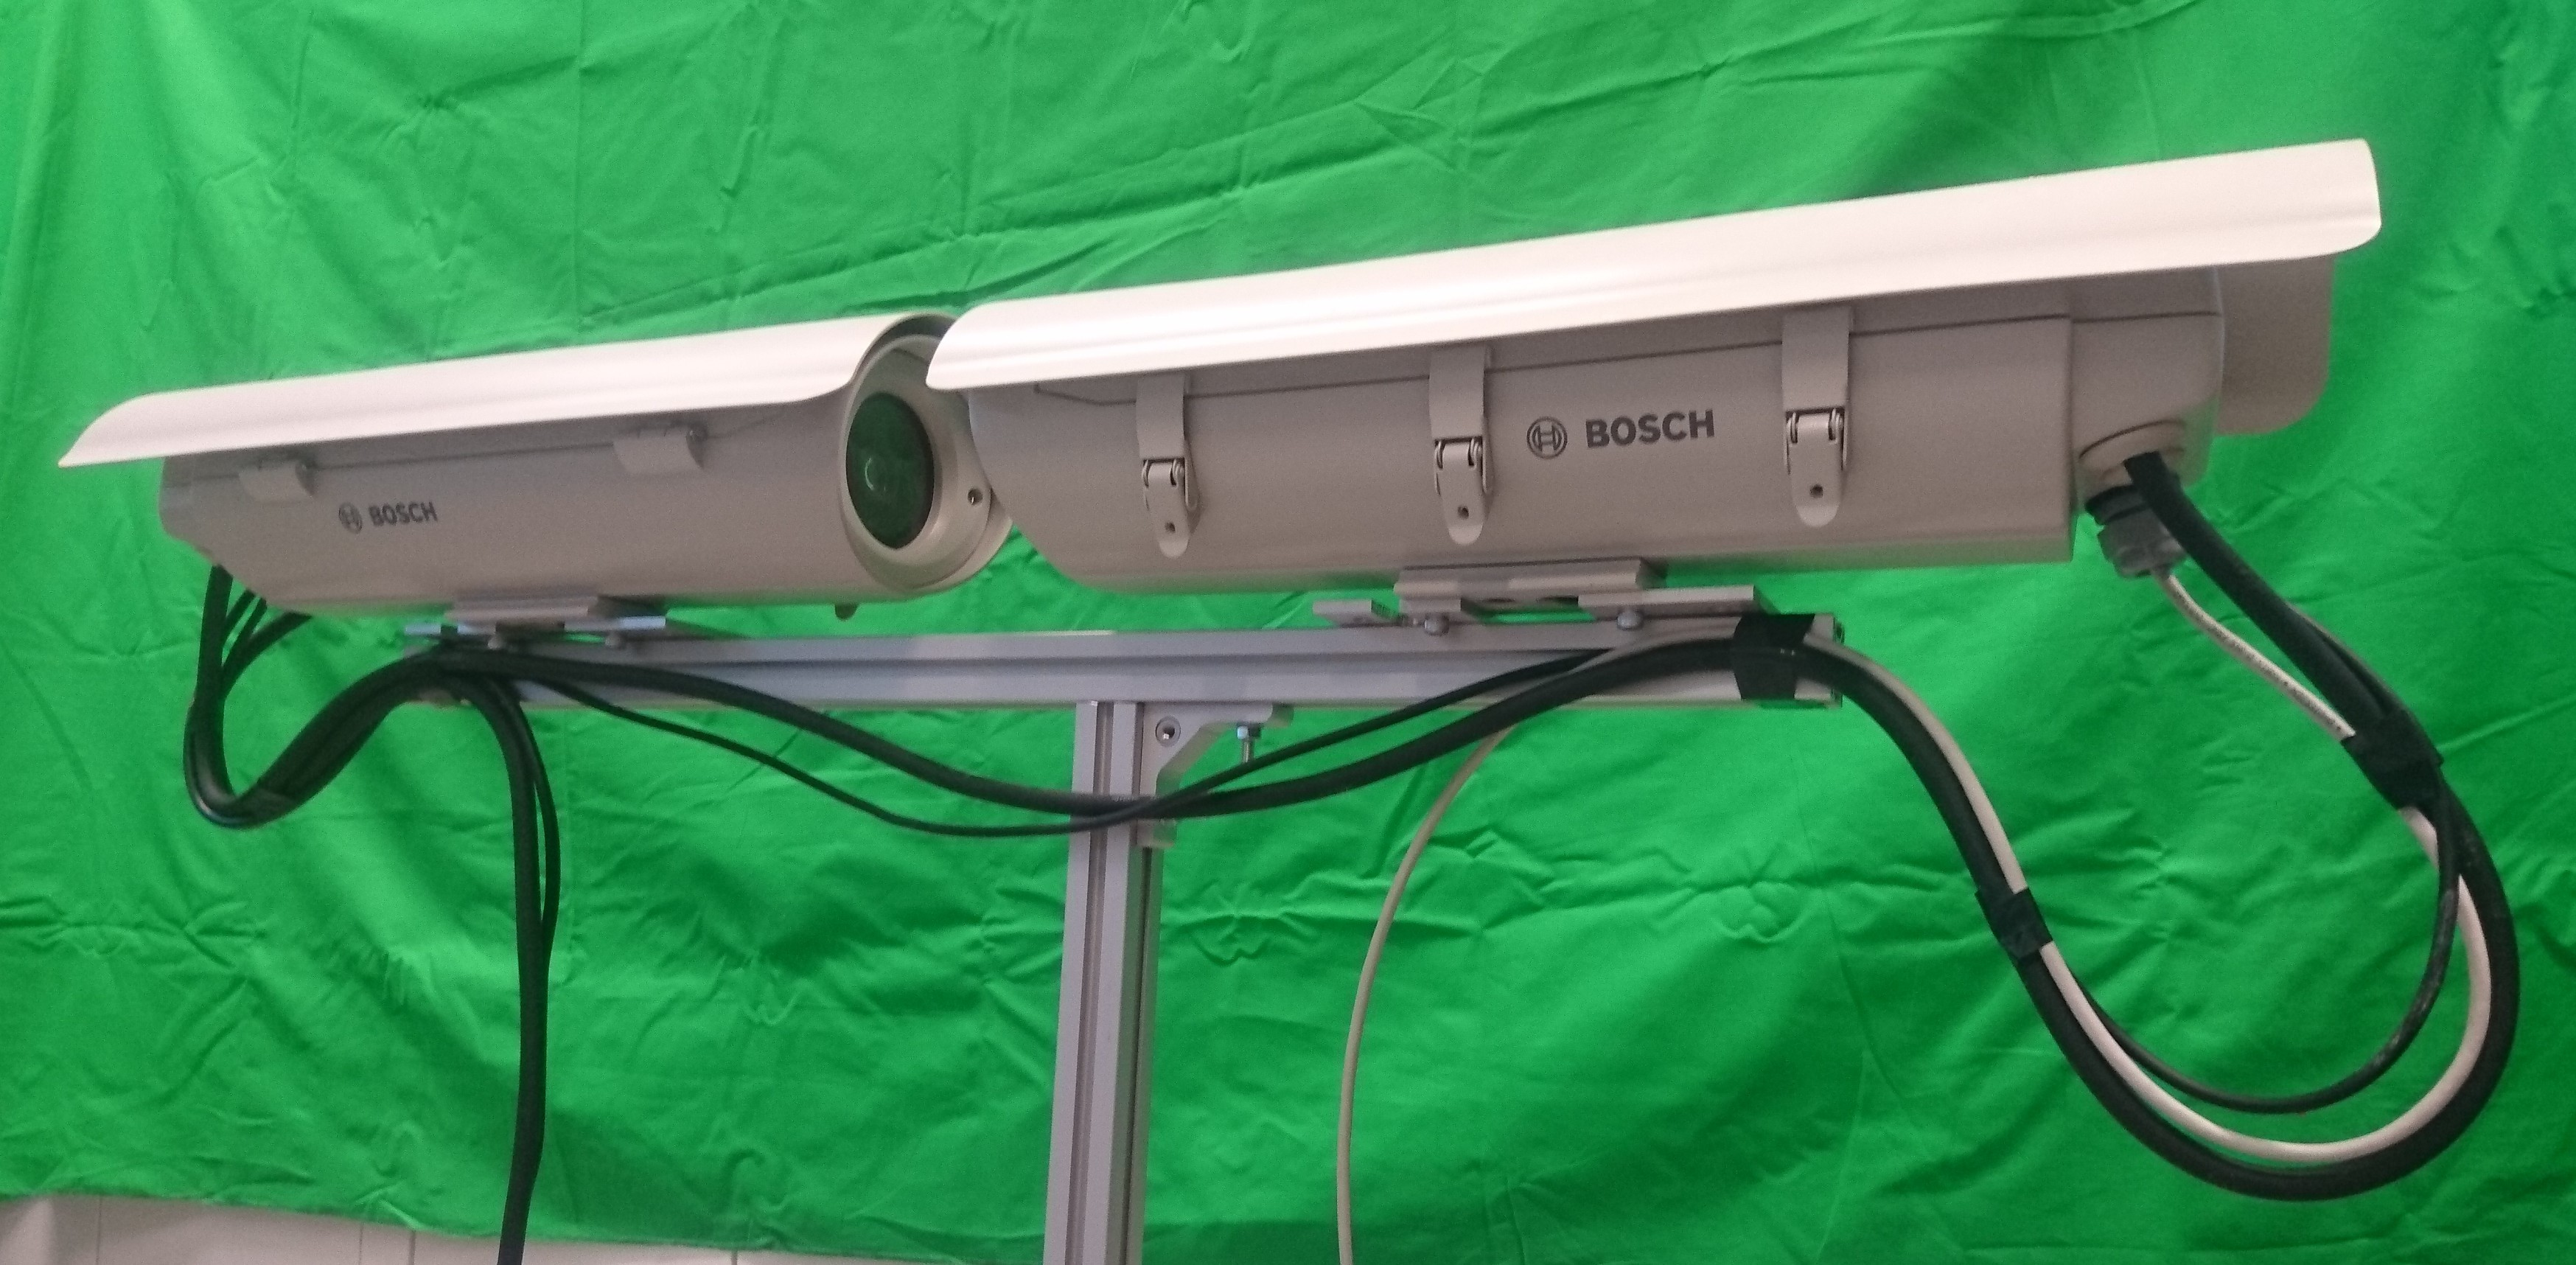
\includegraphics[width=0.75\linewidth]{figures/cam_housings}
\caption{The illumination and detector is mounted inside two Bosch camera housings facing each other with heating inside the housings and on the front glass.}
\label{fig:housings}
\end{figure}

\section{Overview and Process}
\label{sec:overview}

\begin{figure}[ht]
\centering\includegraphics[width=0.75\linewidth]{figures/El_interfaces}
\caption{Electrical interfaces and system overview.}
\label{fig:el_if}
\end{figure}

A stage micrometer scale was used for characterization of the system and simulation of water droplets. This characterization holds true given that the optical silhouette of a droplet is comparable to a dot of equal diameter printed on a silicon glass. It is not a new concept and has been proved experimentally by comparing beads of glass and water droplets of known sizes \cite{koro1991,koro1998}. Light passing a transparent sphere is affected by its refraction, reflection, diffraction and absorption. Of these four components, the shadow will be defined mainly by the diffracted, as long as the distance between the sphere and the lens is much greater than the sphere's diameter \cite{koro1991,wend2013}.

The design using a weakly collimated \gls{led} that illuminates an area slightly larger than the field of view makes the system quite insensitive to misalignment of the camera and the light source. Temporal or permanent changes in light intensity caused by a minor misalignment are automatically compensated for by continuous measurement of the total exposure level. If the level of exposure is increasing or decreasing, the length of the light pulse is changed correspondingly. The light intensity can also be affected by dirt on the front glass of the housings. 

Since many images do not contain any droplets at all, we increase the processing speed by sorting out the images that do not contain any interesting information. This is done by constructing an average image from 20 images. All new images are compared with this average, and if any pixel differs from the average, by more than a specific value that is significantly higher than the noise level, the image is analyzed. The average image is re-constructed periodically.

Spatial dissimilarities in the light intensity that are not caused by noise are compensated for by calculating the local average intensity of the background around each measured droplet. This way, a variable threshold \cite{gonz2002} is constructed.The size of a droplet is then based on the intensity dip caused by the shadow compared with its local background.

\begin{figure}[ht]
\centering\includegraphics[width=0.75\linewidth]{figures/Img_proc}
\caption{Flowchart illustrating the method of image processing step by step.}
\label{fig:img_proc}
\end{figure}

\section{Image Segmentation}
\label{imgsegment}

If the image contains an object detected by the thresholding, the sample volume is calculated for each droplet individually depending on its size. By using a Laplacian of Gaussian \cite{marr1980, gonz2002} edge detection and a suitable threshold, we can create closed curves around objects where the edge is in or near focus. Other edge detection operators like Roberts, Prewitt, Sobel \cite{gonz2002} and Canny \cite{canny1986} did not seem to give the same consistant performance in different lighting conditions. The objects that create closed curves, selected by a boundary fill function, are said to be within the measuring range. The measuring range together with the field of view defines the sampling volume. The measurement volume is described in Paper I. Since the Laplacian of Gaussian can be seen as value of the second derivative of the edge gradient, it is also used together with the diameter to calculate the true size of the droplet. This is described in Paper II.

\subsection{Exposure Check and Flash Intensity Adjustment}

Let $I_{i,j}$ denote the two-dimensional image captured by the camera. The mean value $\overline{i}$ of all pixels in the image $I_{i,j}$ gives an estimation of the exposure level in the whole image. 

The flash duration is adjusted automatically by the microcontroller at each exposure to keep the exposure level between a low and a high threshold, $th_L$ and $th_H$. The duration is changed in steps of 13 ns corresponding to one clock cycle of the microcontroller. If $\overline{i} > th_L$ and $\overline{i} < th_H$ the image is analyzed. If $\overline{i} \geq th_H$ the flash duration is decreased by steps of 12 ns. If $\overline{i} \leq th_L$ the flash duration is increased. The total flash duration is approximately 250 ns. Here $th_L$ is set to 0.7 and $th_H$ is set to 0.8 in a normalized (0,1) dynamic range.

\subsection{Edge Detection and Edge Sharpness}

To detect the intensity changes created by the shadow of a water droplet, an image is processed using the Laplacian of Gaussian (LoG) described by Marr and Hildreth \cite{marr1980}. The method works by looking for zero crossings in the image resulting from calculating $\nabla^2 G\left(x,y\right) * I\left(x,y\right)$. $G\left(x,y\right)$ is a two-dimensional Gaussian distribution with standard deviation σ and $\nabla^2$ is the Laplacian operator, defined as the divergence of the gradient in two dimensions.
\begin{equation}
G\left(x,y\right) = \frac{1}{\pi \sigma^2} e^{-\frac{x^2+y^2}{2\sigma^2}}
\end{equation}
\begin{equation}
\nabla^2=\nabla\cdot\nabla=\frac{\delta^2}{\delta x^2} + \frac{\delta^2}{\delta y^2}
\end{equation}
We implement a discrete approximation to $\nabla^2 G\left(x,y\right) \approx \nabla^2 G_{i,j}$ as a 13x13 sized convolution kernel.
\begin{equation}
\nabla^2 G_{i,j} = -\frac{1}{\pi \sigma^4} \left(1 - \frac{i^2+j^2}{2\sigma^2} \right) e^{-\frac{i^2+j^2}{2\sigma^2}}
\end{equation}
By applying the convolution to the normalized image $I_{i,j}$ we get the image $P_{i,j}$.
\begin{equation}
P_{i,j}=\nabla^2 G_{i,j} * I_{i,j}
\end{equation}
$P_{i,j}$ is thus a matrix that contains the second order derivative of the image $I_{i,j}$. 
A spherical object will result in an edge where the intensity change is similar around a spherical object, but dependent on the distance from the optimal focus. Assuming the Gaussian of the image I is twice differentiable at any point $(i,j)$, the maximum (or minimum) of the second derivative includes the amplitude of the first derivative at the point where the second derivative is equal to zero, i.e. where the edge is strongest. This can be intuitively understood; when the edge is sharper, the gradient, or first derivative value, is larger. And if the gradient value is larger, the rate of change, i.e. the second derivative, needs to be larger at each side of the edge. Therefore, we store a value of the maximum second derivate, $max(P_{i,j}$), around each analyzed object and use this as a measure of the edge sharpness. This value in turn is used as input to a calibration function. 
We also construct a new binary image $Q$ in which the pixel value $Q_{i,j}=1$ if any of $|P_{i+1,j}-P_{i,j} |,|P_{i-1,j}-P_{i,j} |,|P_{i,j+1}-P_{i,j} |,|P_{i,j-1}-P_{i,j} |>th$, where $th=0.002$. $Q_{i,j}=0$ elsewhere. th is the gradient of the second derivative at the point where the second derivative is zero, i.e. on the edge. Particles are found by searching for closed contours in this binary image.

\subsection{Comparing Transparent Microspheres and Dots}

A spherical lens scatters almost all the incident light in different directions, leaving only a bright spot in the middle where the light is transferred directly through. For larger particles in focus, this bright spot can result in a second circular closed contour inside the outer edge. 

Small water droplets can be seen as transparent microspheres. The composition changes the refractive index, but this has little effect on the shadow. The outer contour is the same following the same reasoning as dots used for calibration in Paper I. Diffraction patterns depend on the wavelength of the light and the size of the sphere. The resolution of the constructed system is not high enough for these patterns to be visible.

By using a flood-fill function on the binary image containing the detected contour, starting at a point at a minimum distance from an object, the edge of the filled area will border to the outer contour. This makes it possible to select the outer closed contours of possible particles.

\subsection{Removing the Center Bright Spot}

The center bright spot will make the shadow of a transparent sphere brighter in average than a solid dot. This will have an impact on the size calculation, since the size calculation is based on the shadow impact and the calibration is done using solid dots. Therefore, we apply a mask on the image before calculating the size of the shadow. The mask is done by replacing all the centermost pixels in the shape of a circular disc with the intensity of the darkest pixel in the spot. The diameter of the masked disc is the arc length of the edge contour divided by $\pi$. The bright spot is measured by calculating the difference between the least value and the center pixel. Only particles with a difference greater than 0.1 (ten percent) will have the mask applied

\subsection{Measuring Roundness}
\label{met:roundness}
There may be clogs of small microspheres or dust in the samples that are measured. Microspheres, or small water droplets are close to spherical. We try to exclude all objects that the program finds that are not circular. After the detection of object edges, we measure the roundness of each object. A measure of the mean square roundness deviation similar to the one described by ISO \cite{iso12181} can be achieved by calculating the quote between the area of the contour and the square of the total arc length. See (\ref{eq:5}).
\begin{equation}
roundness = 4\pi \frac{A_{contour}}{arcLength^2}
\label{eq:5}
\end{equation}
$A_{contour}$ is the pixel area of the filled contour and $arcLength$ is the perimeter of the measured closed contour. In the calibration and field measurements described, an object is only considered spherical if $roundness \geq 0.85$.

\section{Light Source}

Although water is a good absorber of electromagnetic radiation in most spectral wavelenghts except for the visible, the volume of water droplets is too small for the absorbtion to be measurable. In visible light, the water droplet can be regarded as a spherical lens with a very short focal length, thus spreading most of the light in diverging directions. Since the camera used is designed for both visible and near infrared light, we tested and compared two different wavelenghts, 455 nm and 850 nm using the same optical setup. The shorter wavelength gave sharper images and higher \gls{snr}.

\begin{figure}
\centering
\begin{minipage}{.5\textwidth}
  \centering
  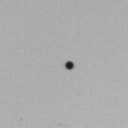
\includegraphics[width=.6\linewidth]{figures/compare455nmdot}
  %\caption{A subfigure}
  %\label{fig:compare455nmdot}
\end{minipage}%
\begin{minipage}{.5\textwidth}
  \centering
  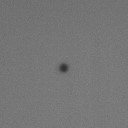
\includegraphics[width=.6\linewidth]{figures/compare850nmdot}
  %\caption{A subfigure}
  %\label{fig:compare850nmdot}
\end{minipage}
\caption{The same dot viewed with different background light: 455 nm (left) and 850 nm (right).}
\label{fig:comparedots}
\end{figure}

\subsection{Laser Light}

For conventional imaging of small particles the coherence of laser light mainly causes problems as diffraction patterns will be strong and visible. Therefore this was only briefly investigated. In section \ref{sec:discussionlaser} there is a discussion of the result from this investigation.

\subsection{Ambient Light}

In daylight, there is always some ambient light. Although the camera is never aimed direclty at the sun and has a telecentric lens, we wanted to be sure that this light would not affect the measurement. For an indication the amount of ambient light, the system was tested in daylight, using a fog generator in front of the lens to reflect light into the lens. 

\section{Image Noise}

We had an idea that it should be possible to measure the signal to noise relation, if the shadow image of the droplet represents the signal. In theory, the \gls{snr} could be used as an input to the size or concentration calculation, to increase the accuracy of the measurement. 

An estimation of the image noise in the whole image was done by making a number of images using only the background illumination. The standard deviation was calculated in each pixel of the 2048x2048 sized image, resulting in an average variation coefficient of about nine percent.

A function was created that calculates the noise level locally around each analyzed droplet image. Assuming that the area surrounding a droplet is evenly illuminated, the SNR can be estimated for each droplet $j$, as the relation between the signal and the ambient noise. The signal is the light amplitude, A$_j$, and the noise is the standard deviation of the surrounding noise, $\sigma_j$. See (\ref{eq:snrcalc}) and \Cref{fig:snrcalc}.

\begin{equation}
snr_j = 20 log \frac{\text{A}_j}{\sigma_j}
\label{eq:snrcalc}
\end{equation}

\begin{figure}%[ht]
\centering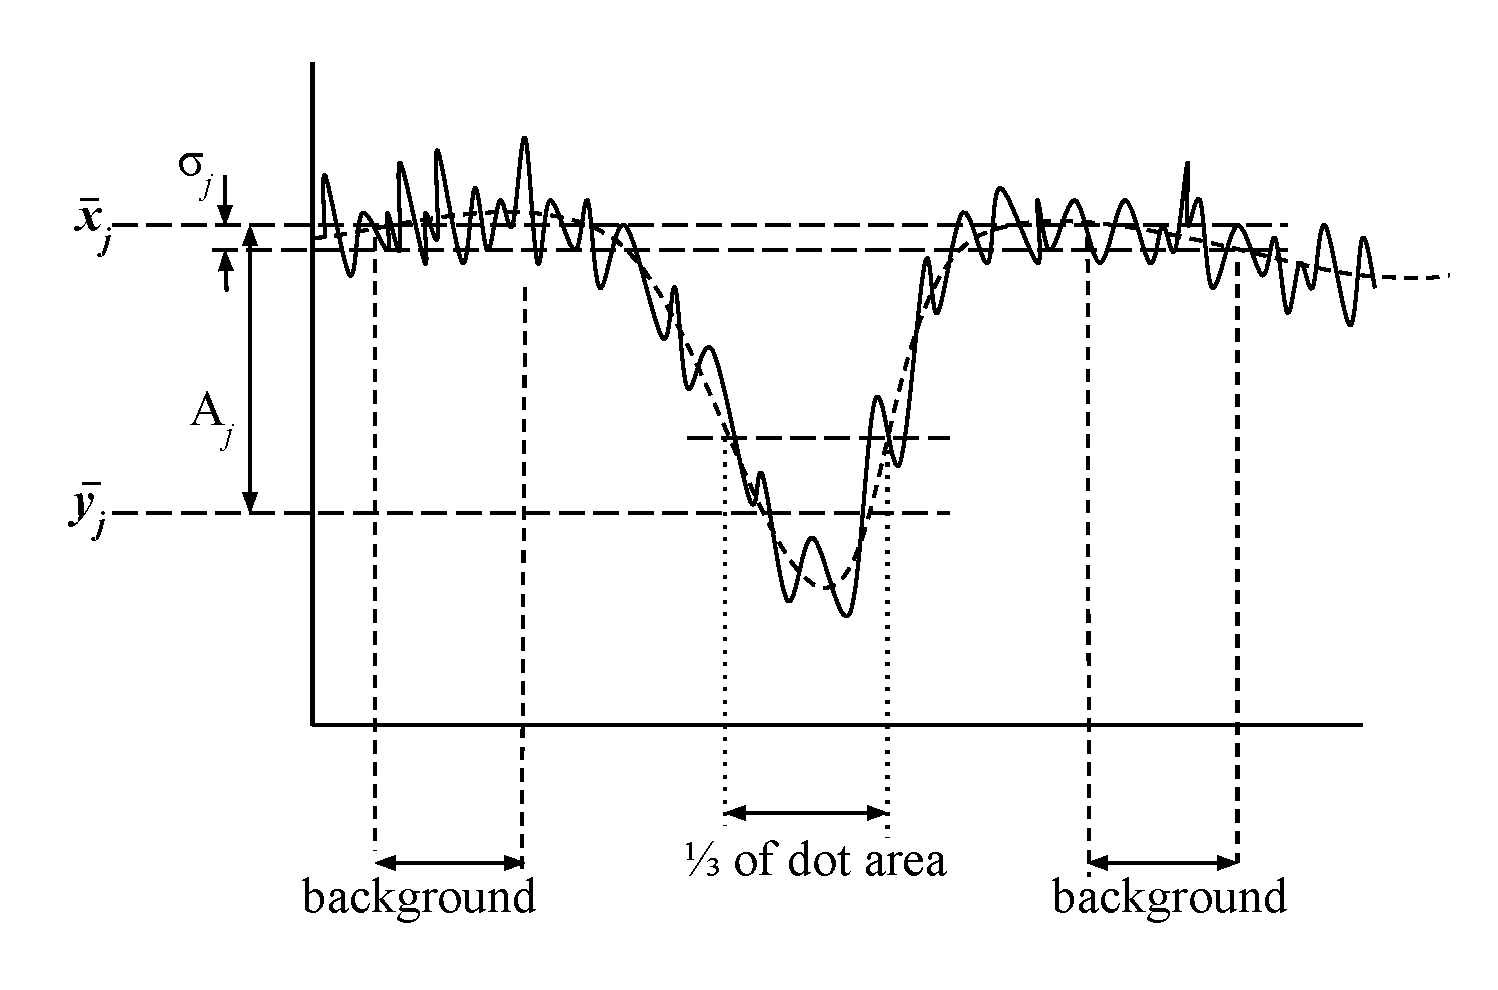
\includegraphics[width=0.75\linewidth]{figures/snrcalc}
\caption{Calculation of the SNR. $\overline{y}_j$ is determined by calculating the average of the darkest third of all pixels inside the edge detected dot.}
\label{fig:snrcalc}
\end{figure}

%\subsection{Exposure Energy Measurement}
%
%This measurement was done to get an idea about the theoretical minimum amount of energy required for each image. In practice, the light from the collimated LED used will be spread so that only a small part of the total emitted energy actually reaches the sensor. The area in view is about 8 times smaller than the illuminated area of the collimated LED, which was measured to about 8x8 mm. Some of the light energy will be absorbed in the telecentric lens.
%
%The light energy required for good exposure was investigated using eight gain setting levels. A pulsed signal was used, 3-10 μs long, with 9-36 kHz frequency. To minimize the thermal effect of the heated glass and the ambient light, the power was measured immediately before and after start and stop. The pulse length was measured using a semiconductor light sensor connected to an oscilloscope. The result is discussed in section \ref{sec:expmeasurement}.


\section{Calibration and Validation of the Calibration}

Because of the diffraction, the edge of an object is difficult to measure directly by thresholds, even if the coherence length of the light is small and the object is in focus. The edge will apprear blurry. For objects out of focus, the blurring will increase even more. Therefore the size measurement is calibrated by both measured diameter and a value of the edge sharpness, or gradient.

Also the measuring range needs to be calibrated. The measuring range is here defined as the distance in which the edge detection by Laplacian of Gaussian operator and a threshold makes a closed curve in the resulting binary image. This will be different especially for smaller objects.

The system was calibrated using a stage micrometer scale with 13 circular dots printed in chrome on a silicon glass. The dots range from 2 to 100 μm in diameter. Each dot was moved linearly in steps of one micrometer in the direction orthogonal to the lenses, thus creating a function where the gradient of the edge depends on the distance from optimum focus. A threshold on the second derivative gradient strength limits the measured particles to be within a specific measuring range. The threshold should be selected carefully. If the value of the threshold is too low, there will be many false edges in the image. If it is too high, the measuring range will be too small. The difference between two different thresholds, 0.002 and 0.005 is illustrated by \Cref{fig:measrangevslogth}. The lower threshold was used in the following measurements.

\begin{figure}[ht]
\centering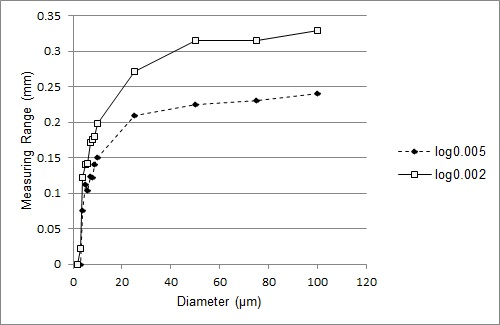
\includegraphics[width=0.75\linewidth]{figures/meas_range_vs_log_th}
\caption{Measuring range (mm) vs. diameter for two different thresholds (0.005 and 0.002).}
\label{fig:measrangevslogth}
\end{figure}

The edge sharpness will affect the position of the edge and the measured shadow slightly. We use the maximum value of the second derivative $P_{i,j}$ for each droplet as a measure of the edge sharpness and include this in the calibration functions, together with the diameter measured from the shadow intensity.

Two second degree approximation surfaces, (\ref{eq:z1}) and (\ref{eq:z2}), are calculated using the “fit” command in Matlab. $z_1$ approximates dot diameters from 2 to 10 micrometers and $z_2$ diameters from 10 to 100 micrometers. x is the maximum second derivative, $d^M$ is the diameter measured from the shadow intensity, $p_{xx}$ and $q_{xx}$ are constants.

\begin{equation} \label{eq:z1}
z_1=p_{00}+p_{10} x+p_{01} d^M+p_{20} x^2+p_{11} xd^M+p_{02} {(d^M)}^2
\end{equation}
\begin{equation} \label{eq:z2}
z_2=q_{00}+q_{10} x+q_{01} d^M+q_{20} x^2+q_{11} xd^M+q_{02} {(d^M)}^2
\end{equation}
By measuring the calibrated microspheres a validation can be made with the expected diameter. 

\subsection{Verification of Dot Size}

The dots on the micrometer scale were measured visually using a Leica microscope connected to a digital camera. This was done to find accurate values of the diameter of the dots to use in the calibration. An example image that was measured can be seen in \Cref{fig:50umdot40x}.

\begin{figure}[ht]
\centering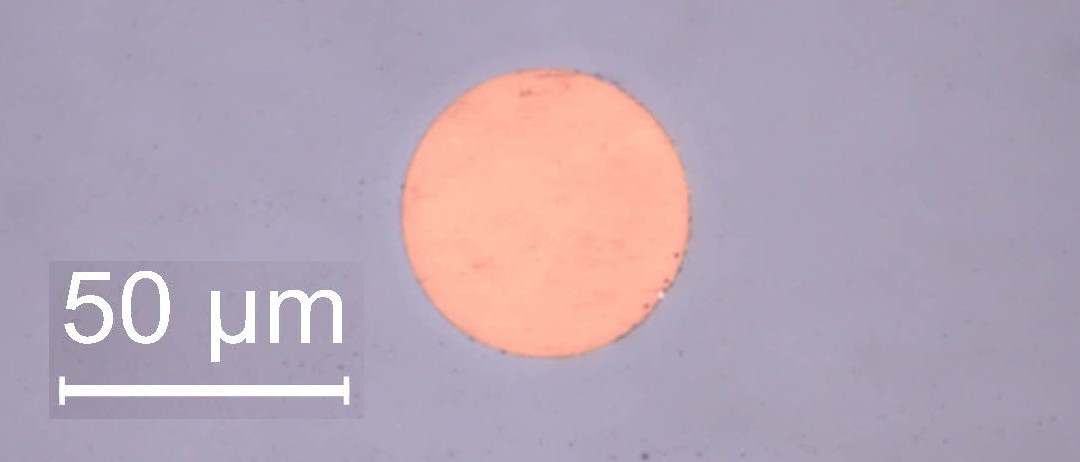
\includegraphics[width=0.75\linewidth]{./figures/50umdot40x.jpg}
\caption{The 50 micrometer dot with front illumination imaged using 40x magnifying lens.}
\label{fig:50umdot40x}
\end{figure}

This measurement was done using lenses with two different magnifications: 40x and 100x. All the dots average diameters, except the 100 µm dot were found to be within $\pm$0.2 $\mu$m of their nominal diameter. They are not all perfectly round, but the size accuracy should be good enough to use as calibration reference. The result from this measurement is presented in \Cref{tab:ref_meas}.

\begin{table}[ht]
\centering
\begin{tabular}{p{0.2\linewidth} p{0.2\linewidth} p{0.2\linewidth} p{0.2\linewidth}}
\hline
\textbf{Nominal Diameter} & \textbf{Excentricity} & \textbf{Diam. 40x} & \textbf{Diam. 100x} \\
\hline
5 & 0.2 & 5 & 4.8 \\
6 & 0.6 & 5.8 & 5.8 \\
7 & 0 & 7 & 6.6 \\
8 & 0 & 8 & 7.9 \\
9 & 0 & 9 & 8.8 \\
10 & 0 & 10.1 & 9.8 \\
25 & 0 & 24.9 & 24.7 \\
50 & 0.4 & 50.1 & 49.8 \\
75 & 0.2 & 75.2 & 74.8 \\
100 & 2.5 & 100 & 98.7 \\
\hline
\end{tabular}
\caption{Micro dot verification measurement. All values are in µm. Here, eccentricity is the maximum difference in µm between the smallest and the largest measured diameter.}
\label{tab:ref_meas}
\end{table}



\section{The Fog Chamber}

Natural fogs tend to not coincide with when we are ready to test. The fog chamber was needed to create a test environment for the instrument. 

The constructed chamber has a frame made of 30 mm aluminum profiles, fitted with transparent 6 mm polycarbonate walls on all sides using rubber sealing strips. The droplets are produced using an ultrasonic fog generator pushing the droplets to the chamber through a flexible tube approximately 30 mm in diameter and 500 mm long. Next to the fog inlet, there is a dry air inlet with a speed adjustable fan. On the back of the chamber there is a similar-sized outlet for air and moisture. See \Cref{fig:fogchamber}.

\begin{figure}[ht]
\centering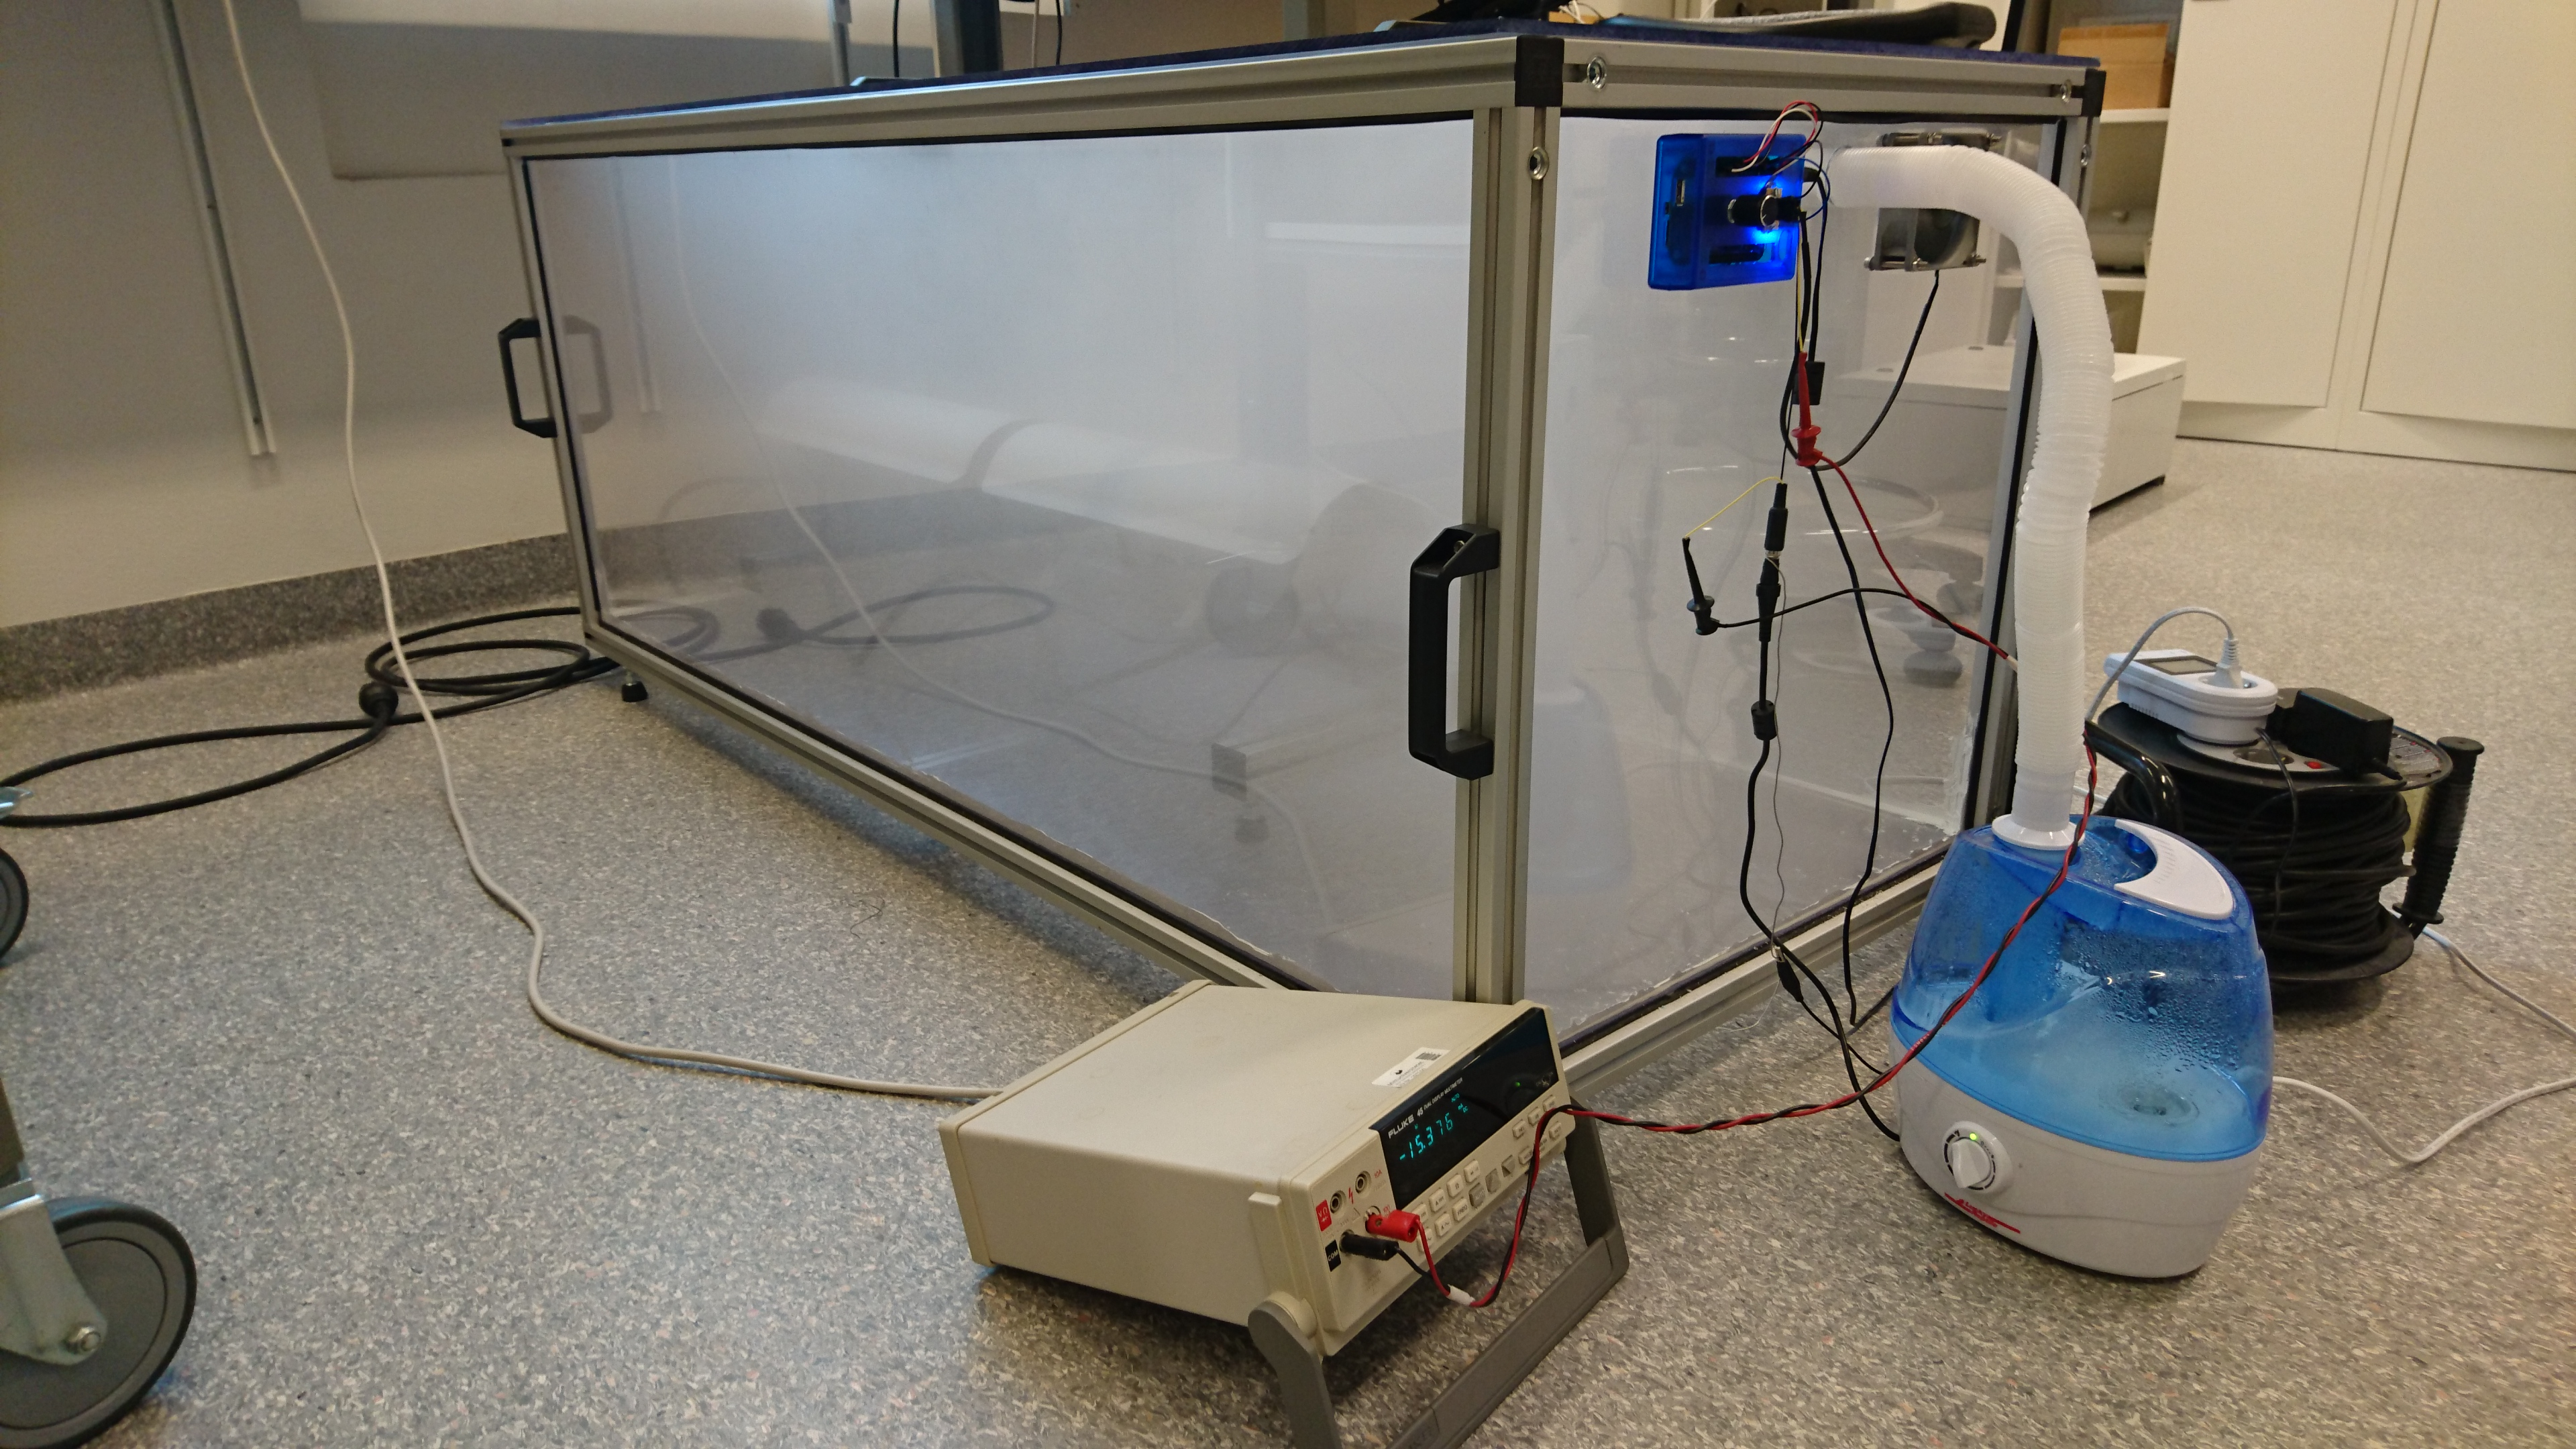
\includegraphics[width=0.75\linewidth]{figures/DSC_0103}
\caption{Fog chamber with connected droplet generator (blue container) and a multimeter used for fan power measurement. A Beaglebone Black microcontroller (blue box) is used for fan speed regulation.}
\label{fig:fogchamber}
\end{figure}
 
Unfortunately, we could not fit a second instrument in the fog chamber for verification of the \gls{lwc}. The \gls{cdp} requires an airflow with a known speed to be able to calculate the particle concentration. The fog chamber worked very well as a functional test and a verification of the instrument’s water ingress resistance.

\section{The Klövsjö Installation}

\Cref{fig:installation1} shows a complete installation of the DII and the \gls{cdp} at the Klövjö mountain. The two camera houses of the DII are placed on the top, and the smaller \gls{cdp} right underneath. The Lambrecht Eolos weather sensor is placed to the far left, mounted on an horizontal boom. In the middle, to the right of the Eolos, the mobile communication antenna is located. The top of the shortened lattice mast can be seen just below the center. Behind the mast, the top of the box containing the DII processing computer, the \gls{cdp} data collection computer, and the communications router can be seen. The whole installation is about five meters high. An electric servomotor mounted at the base of the pole inside the lattice mast rotates the two instruments automatically to follow the horizontal direction of the wind. 

\Cref{fig:installation3} shows a mix of ice and snow on the front side of the installation.

\begin{figure}[ht]
\centering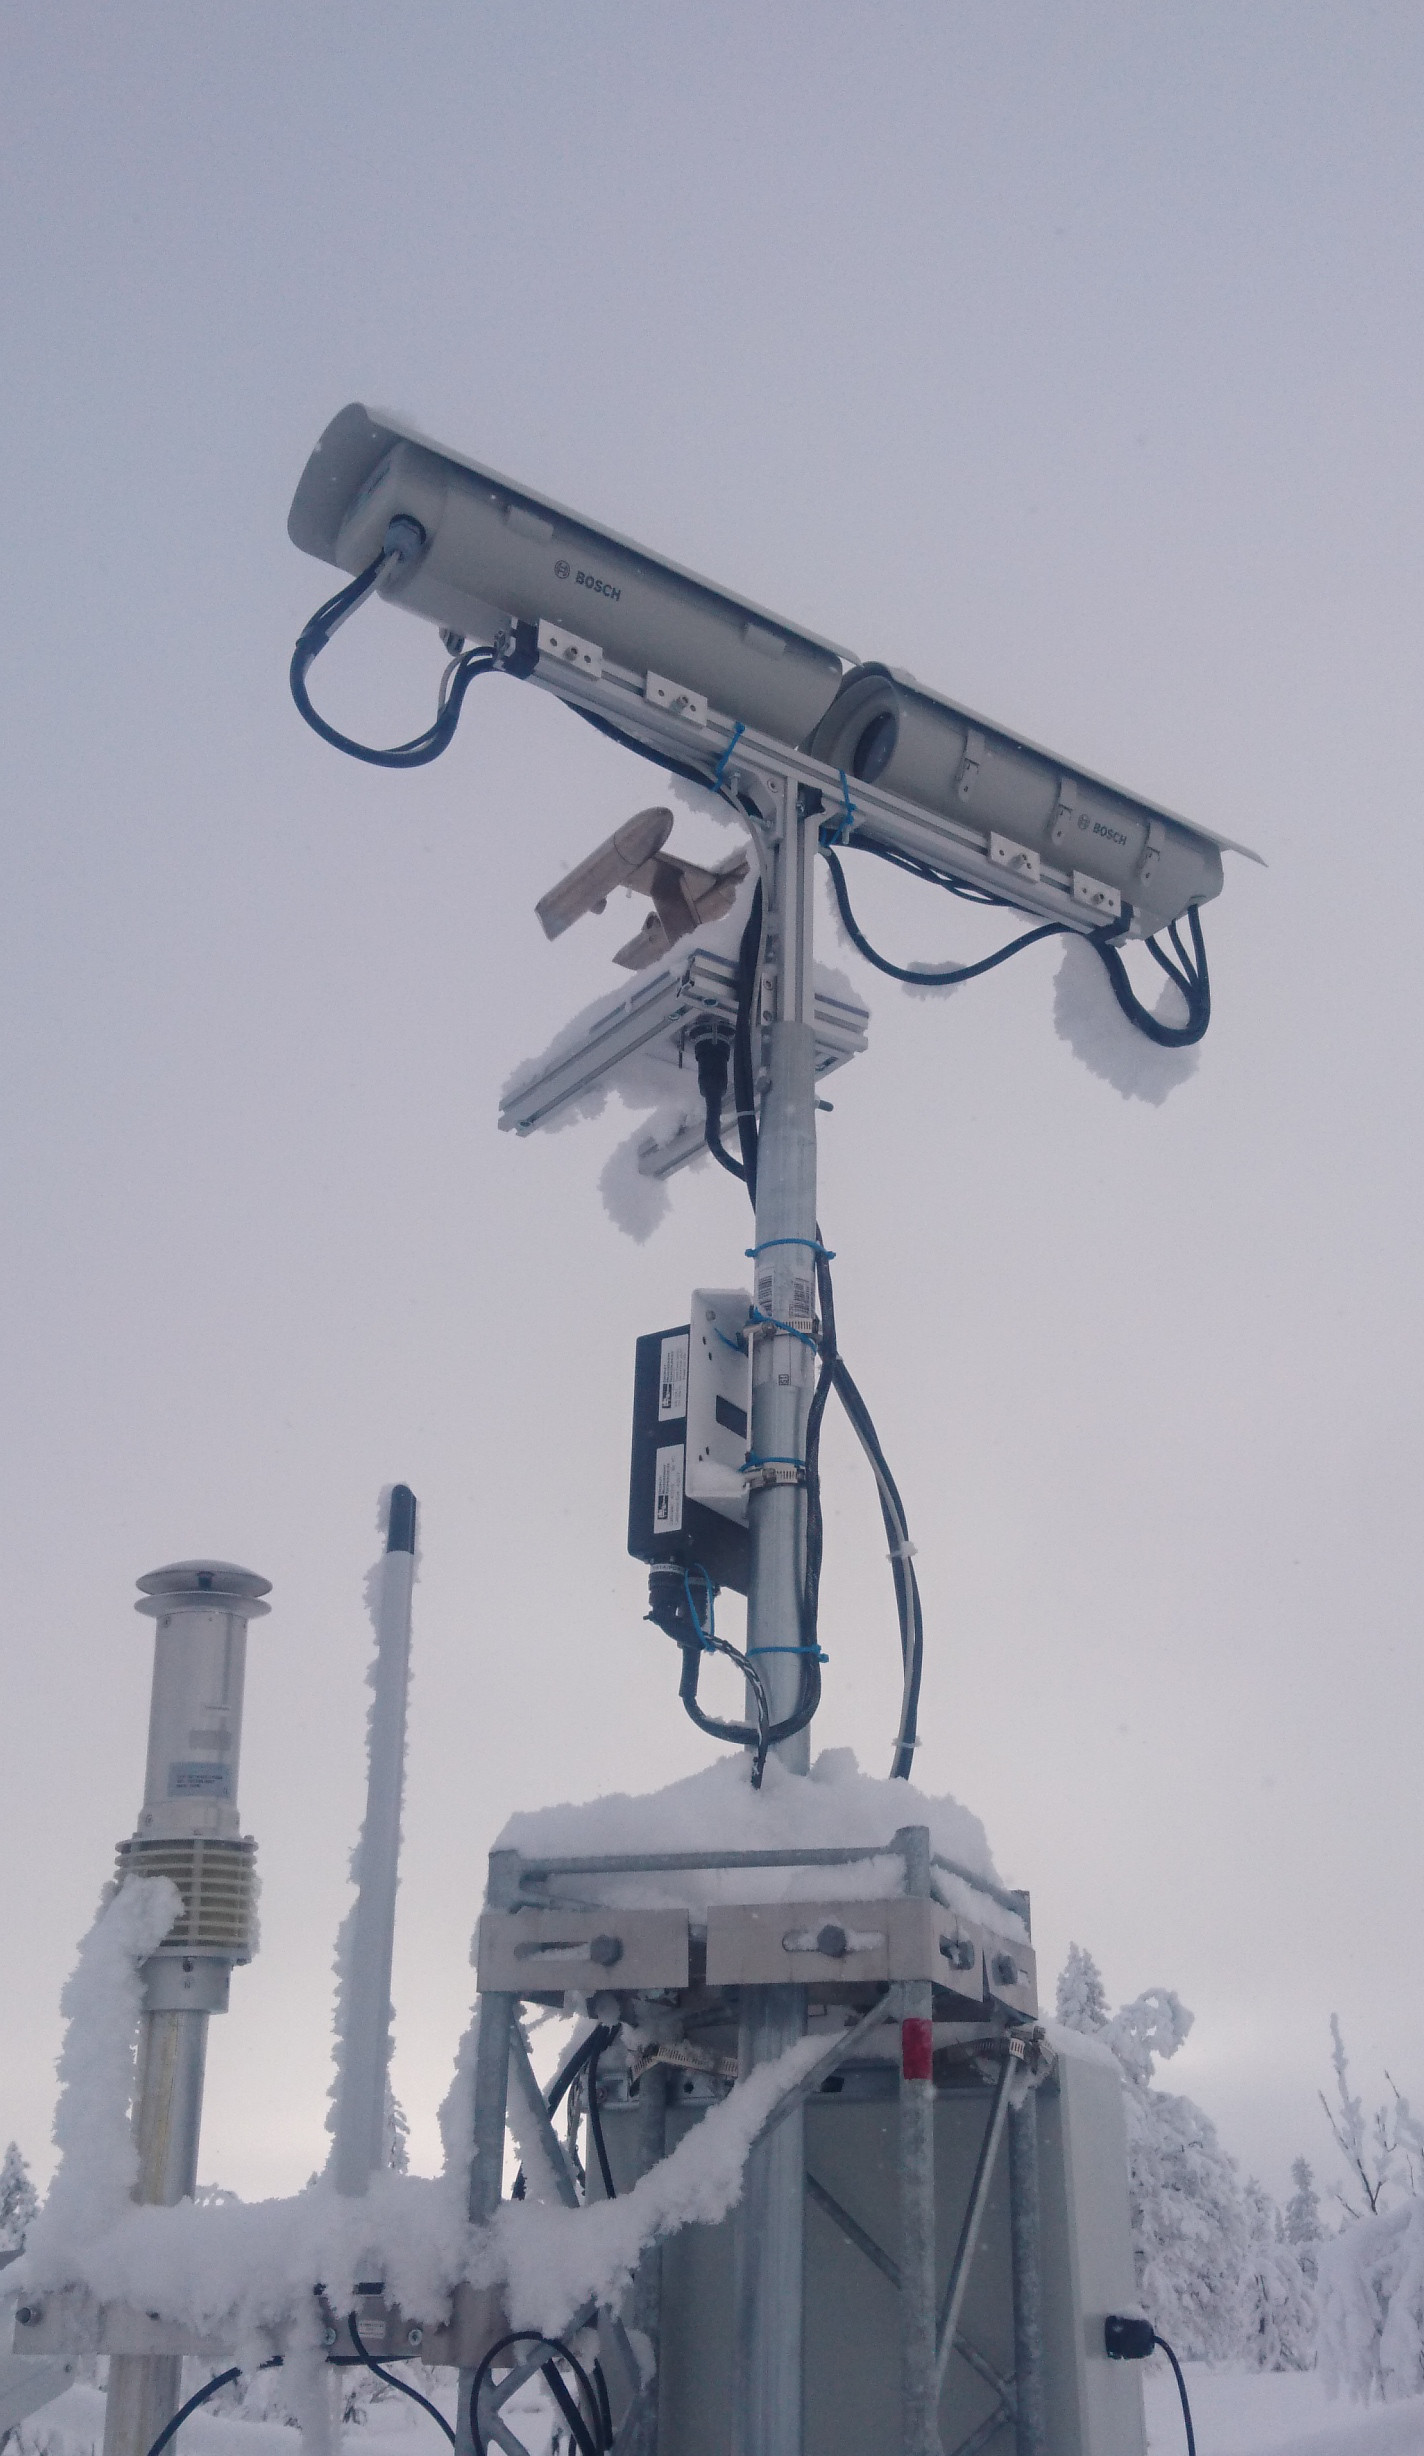
\includegraphics[width=0.75\linewidth]{figures/installation1}
\caption{Installation in Klövsjö.}
\label{fig:installation1}
\end{figure}

\begin{figure}[ht]
\centering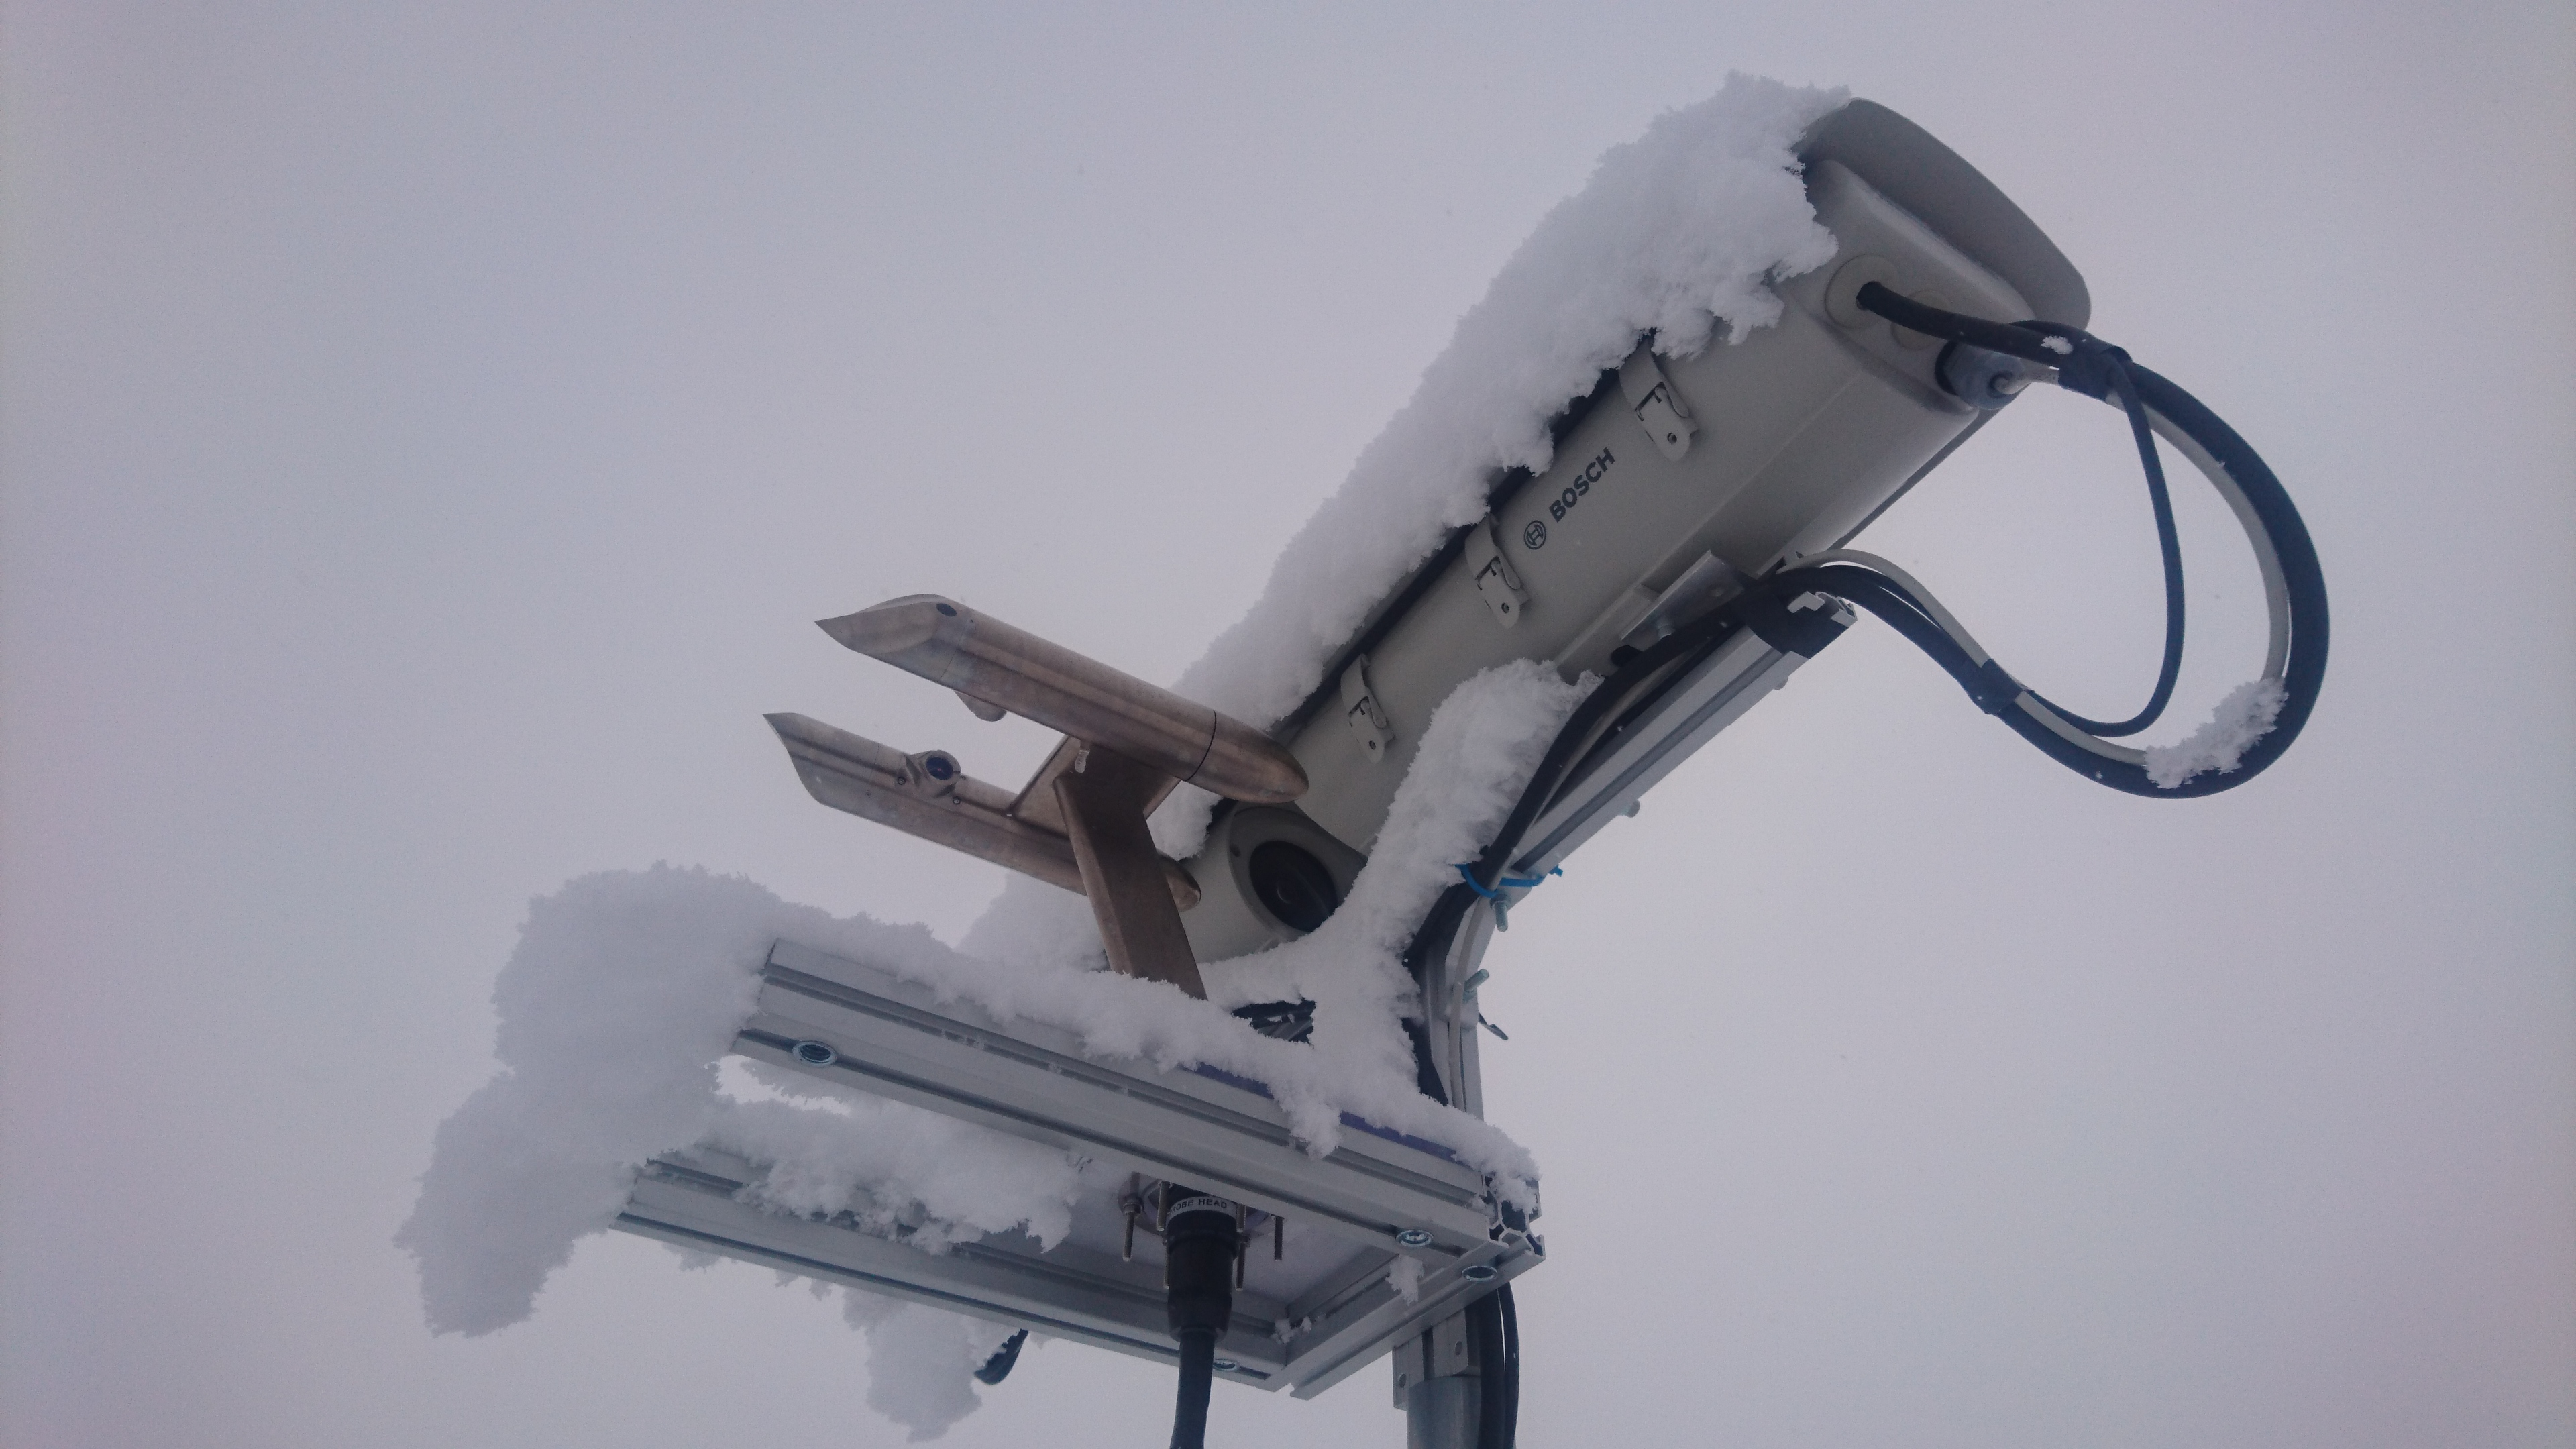
\includegraphics[width=0.75\linewidth]{figures/installation3}
\caption{Ice and snow on the front side of the installed instruments. The CDP is more efficient at preventing ice.}
\label{fig:installation3}
\end{figure}

\section{Numerical Weather Prediction}

For a second validation, we carry out weather simulations around the site using the \gls{harmonie}-\gls{arome} numerical weather prediction (\gls{nwp}) model. The model is described in Paper III.

\gls{smhi} agreed to run a special model domain locally with 500 meters horizontal resolution for a limited time. The operational forecasts are run at 2.5 km horizontal resolution, and they were used as initial conditions and lateral boundaries for the detailed simulations.

At \gls{smhi}, the \gls{harmonie}-\gls{arome} model is used for short range operational forecasting. It is run in cooperation with the Norwegian Meteorological Institute. The initial conditions and boundaries for the operational forecasts are provided by the \gls{ecmwf} global model.

\begin{figure}%[h]
\centering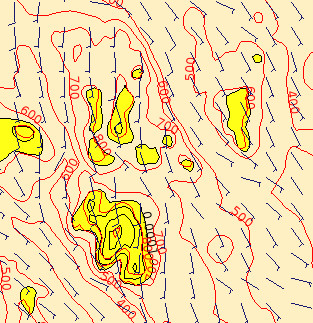
\includegraphics[width=0.6\linewidth]{figures/Images/Klovsjo_smhi160923_small}
\caption{Graphical presentation of data from the HARMONIE-AROME NWP covering Klövsjö and the surrounding mountains at a specific point in time using 500 m resolution. Yellow areas are where the model predicts an LWC more than 0.1 $\mathrm{g \cdot kg^{-1}}$. (Grams of water per kg air.) Simulation and figure by SMHI.}
\end{figure}



% this is shows the paper size and measures
%\begin{figure}
%    \oddpagelayouttrue
%    \twocolumnlayoutfalse
%    \stockdiagram
%    \caption{Right-hand page major layout parameters for
%        the \file{memoir} class} \label{fig:mempplt}
%\end{figure}
%\stockvalues